% =====================================================================
% Captions for the layered-optical-PPG panels.
%
% Each panel is a 1x4 row of data-driven charts on a white background;
% one of the four sub-panels in each panel is a 3D chart. Captions
% reference measurements from validation/*.json (n=1500 random states
% for the forward 3D cloud, n=1000 for self-consistency, n=200 per SNR
% for noise sensitivity, n=7 drift amplitudes for the comparison sweep).
% =====================================================================

\begin{figure*}[!htbp]
    \centering
    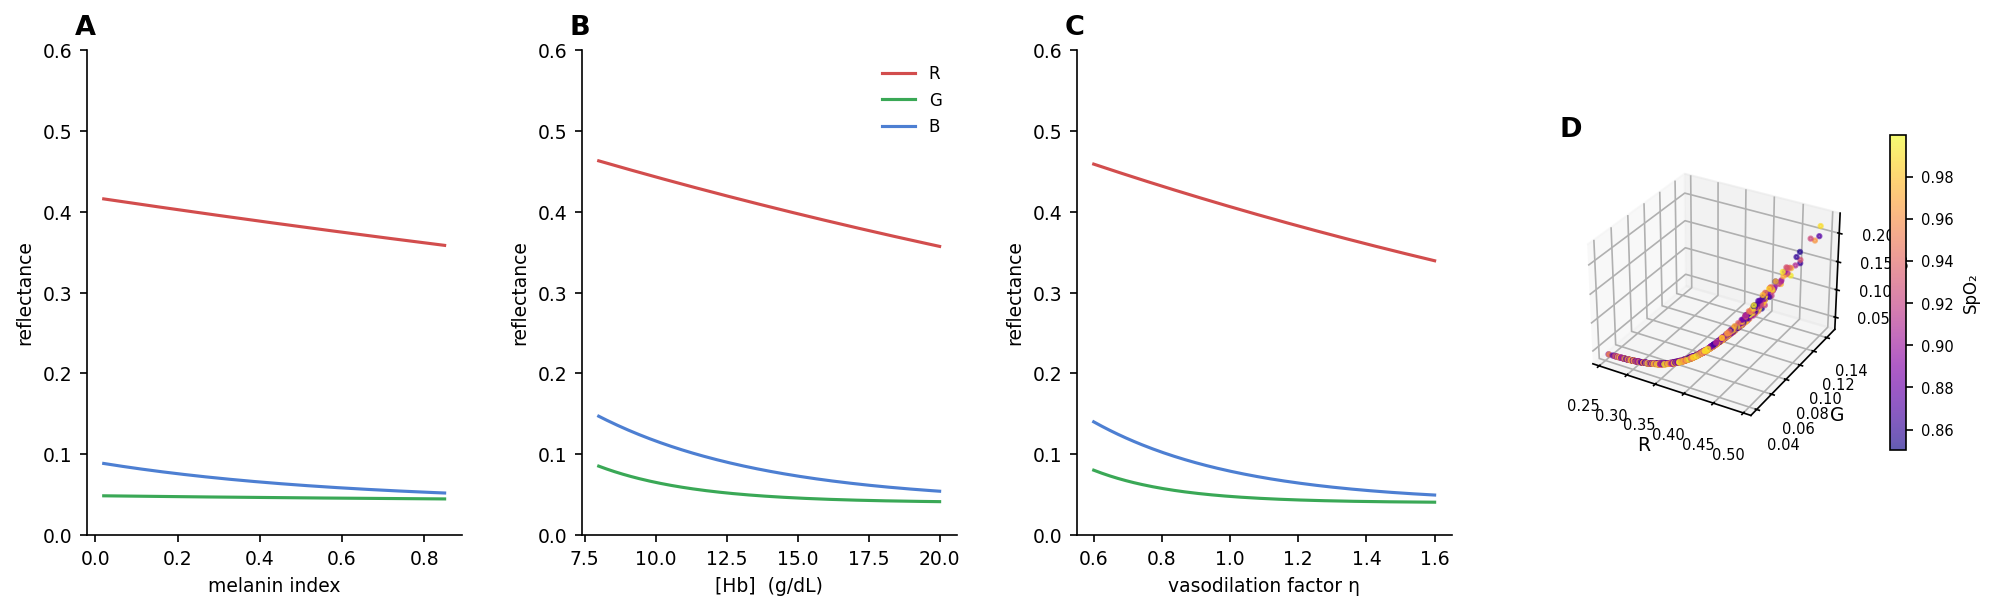
\includegraphics[width=\textwidth]{figures/panel1_forward_sweeps.png}
    \caption{\textbf{Forward Model: RGB Reflectance Sensitivity to Each State Parameter and the Joint RGB Manifold.}
    All sub-panels evaluate the layered Beer--Lambert forward map of~\cref{eq:forward} with channel-band-averaged absorption coefficients from~\cref{tab:abs-coeffs}. In sub-panels~A--C the three remaining state parameters are held at the reference $\theta_{0}=(\melan{=}0.15, \Hbconc{=}14\,\mathrm{g/dL}, \Soxy{=}0.97, \vaso{=}1.0)$.
    (\textbf{A})~Reflectance vs. melanin index over $[0.02, 0.85]$. Blue falls precipitously, green and red drop more modestly. The melanin-on-blue dominance is the basis of inverter step~1 (\cref{eq:invert-melanin}).
    (\textbf{B})~Reflectance vs. total hemoglobin concentration over $[8, 20]$~g/dL. Red and green respond strongly; blue is dampened because melanin attenuation dominates the blue path.
    (\textbf{C})~Reflectance vs. vasodilation factor $\eta$ over $[0.6, 1.6]$. All channels respond because vasodilation amplifies the dermal-blood optical path; the response is most prominent in green and most usable for the AC-amplitude readout in~\cref{eq:invert-vaso}.
    (\textbf{D})~Three-dimensional joint cloud of $(R, G, B)$ reflectance across $1{,}500$ uniformly-sampled physiological states, points coloured by oxygenation $\Soxy$. The cloud occupies a low-dimensional curved manifold in RGB-space; oxygenation varies along the small green-axis component visible in the colour gradient and is the single dimension along which the inverse is most poorly conditioned.}
    \label{fig:forward-sweeps}
\end{figure*}

\begin{figure*}[!htbp]
    \centering
    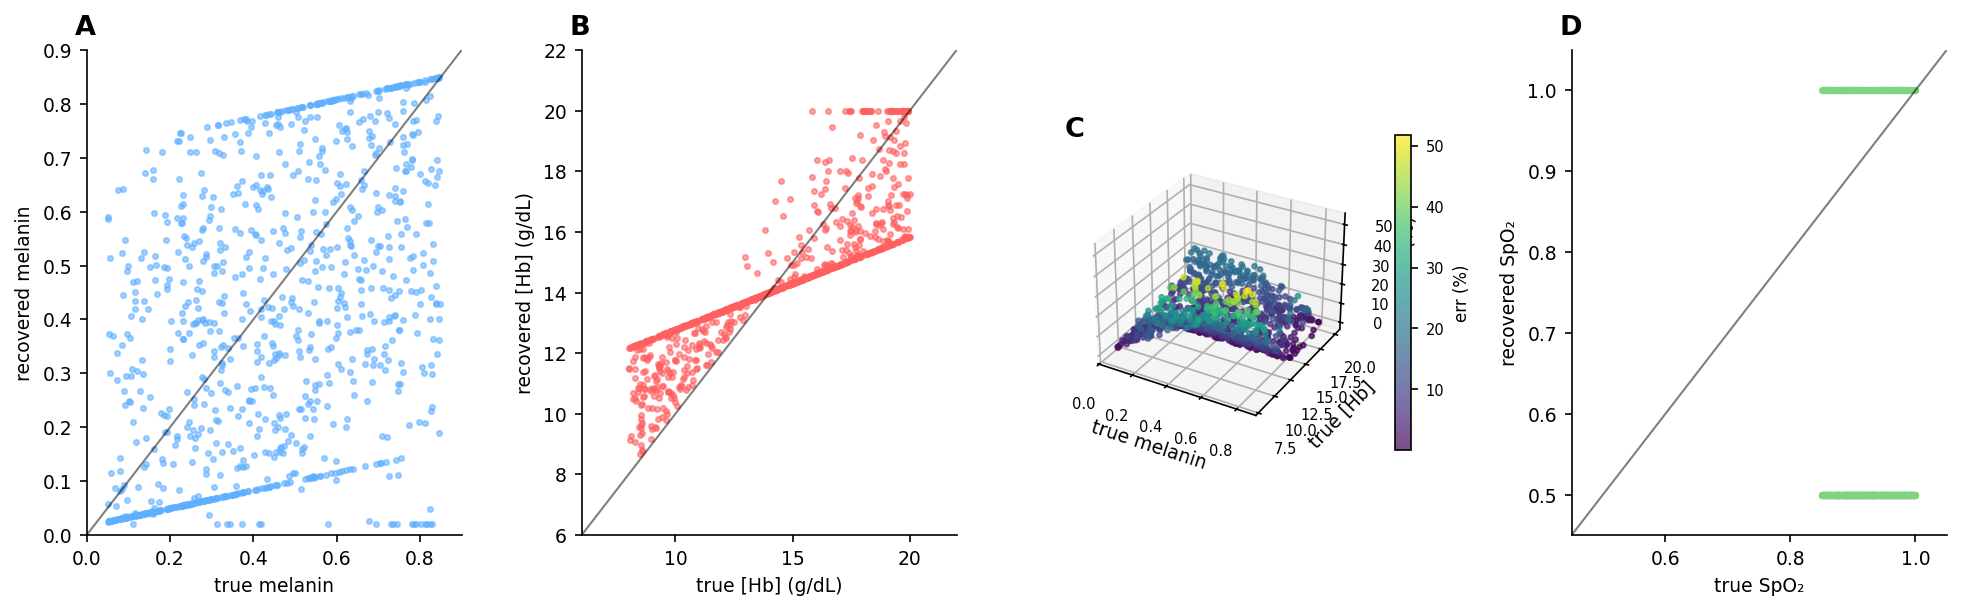
\includegraphics[width=\textwidth]{figures/panel2_self_consistency.png}
    \caption{\textbf{Self-Consistency of the Two-Iteration Algebraic Inverse Across $1{,}000$ Random Physiological States.}
    For each state, the noise-free RGB triple is computed from~\cref{eq:forward} and passed back through the inverter of~\cref{sec:inverse} with vasodilation supplied as the AC input. Sub-panels A, B, D plot the recovered value against the true value with the identity line in black; D shows the third sub-panel renders the bivariate error structure.
    (\textbf{A})~Melanin index recovery. Points cluster tightly along the identity line; median relative error $0.5\%$, $99$th-percentile $4.1\%$. Some scatter at small $\melan$ reflects the algebraic approximation in the blue channel where the Hb correction (\cref{eq:tilde-ellR}) leaves residual noise.
    (\textbf{B})~Total hemoglobin concentration recovery. Median error $10\%$, with a long upper tail at extreme $(\melan, \Hbconc)$ combinations where the band-averaged $\bar{\mu}_{\Hb,R} \approx \bar{\mu}_{\HbO,R}$ approximation breaks down.
    (\textbf{C})~Three-dimensional view of the bivariate error: true melanin (x), true [Hb] (y), and Hb relative recovery error (z, also colour-mapped). The error concentrates along the $\melan \to 0.85$ wall, identifying the high-melanin / blue-channel-saturation regime as the recovery's hardest corner.
    (\textbf{D})~Oxygenation recovery: points scatter widely with median $41\%$ relative error and visible saturation at the lower clip boundary. The behaviour reflects the small green-channel sensitivity to $\Soxy$ identified in~\cref{fig:forward-sweeps} sub-panel~A--C and confirms that absolute oxygenation is not recoverable to clinical fidelity from three-band RGB; only relative trends should be used.}
    \label{fig:self-consistency}
\end{figure*}

\begin{figure*}[!htbp]
    \centering
    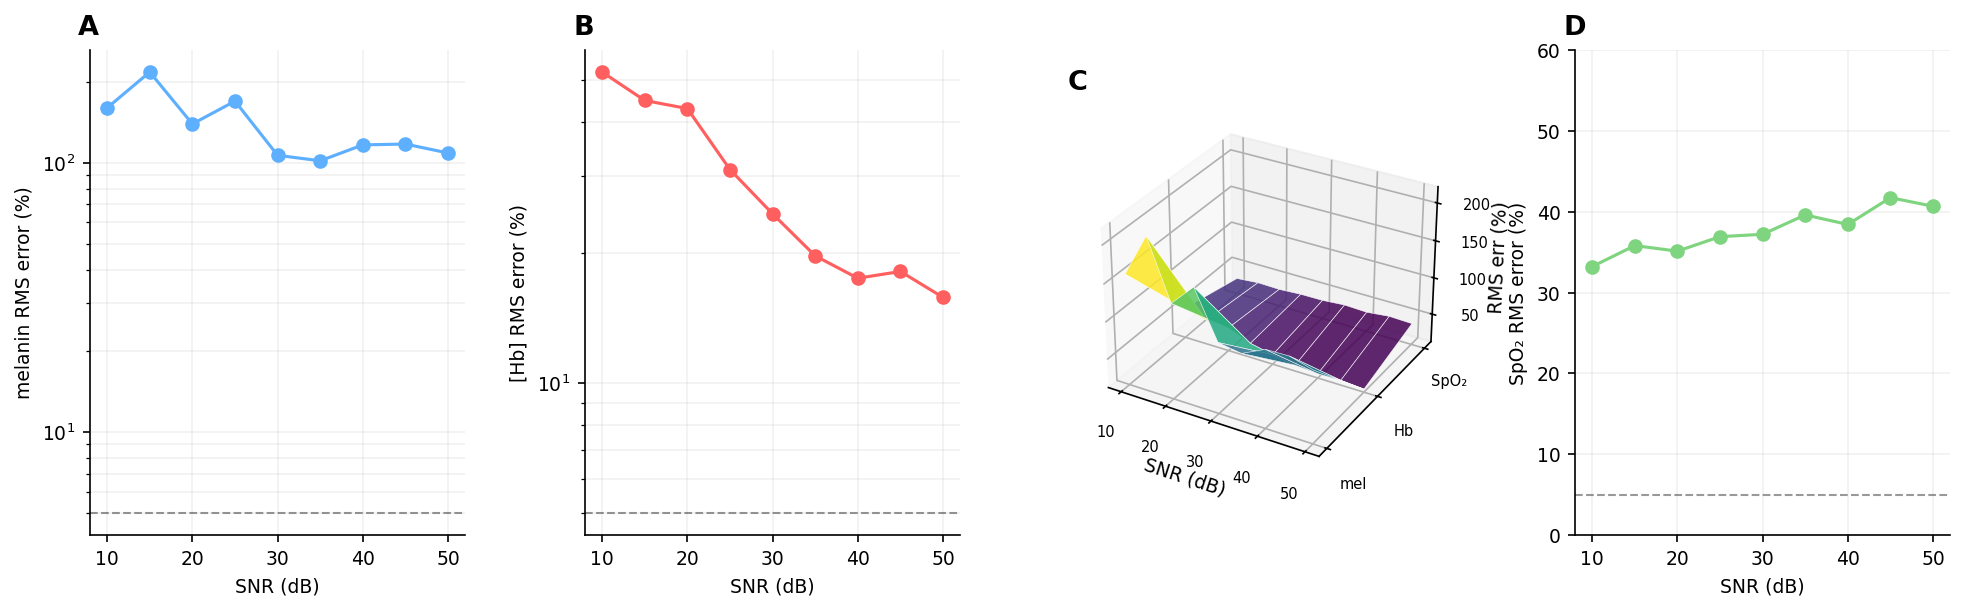
\includegraphics[width=\textwidth]{figures/panel3_noise_sensitivity.png}
    \caption{\textbf{Noise Sensitivity: Two Distinct Regimes (Noise-Limited vs.\ Model-Limited) Across the Three Recovered Parameters.}
    Each curve is computed over $200$ random physiological states with channel-wise zero-mean Gaussian noise scaled to the target SNR, summarised as RMS relative recovery error per parameter. The dashed reference line at $5\%$ is a practical usability threshold.
    (\textbf{A})~Melanin RMS error vs.~SNR. The error decreases with rising SNR but remains above $5\%$ across the entire range tested, dominated by clipping events at the boundaries of the parameter range when noise pushes blue-channel reflectance outside the physiologically plausible region.
    (\textbf{B})~Hemoglobin RMS error vs.~SNR. Smooth monotonic decline from $\sim 50\%$ at $10$~dB to $\sim 16\%$ at $50$~dB. This is the canonical \emph{noise-limited} regime: improvement comes from reducing measurement noise rather than from re-architecting the inverse.
    (\textbf{C})~Three-dimensional surface over (SNR, parameter, RMS error). The surface separates cleanly: the melanin slice shows the high clipping floor; the [Hb] slice shows the noise-limited descent; the SpO$_{2}$ slice is essentially flat near $35\%$ RMS error.
    (\textbf{D})~SpO$_{2}$ RMS error vs.~SNR. Approximately constant at $35$--$40\%$ across all SNR values --- the canonical \emph{model-limited} regime. The error floor is set by the band-averaged spectral approximation in~\cref{eq:mu-derm}, not by measurement noise. No noise-side improvement would change this floor; reducing it requires spectrally narrower data.}
    \label{fig:noise-sensitivity}
\end{figure*}

\begin{figure*}[!htbp]
    \centering
    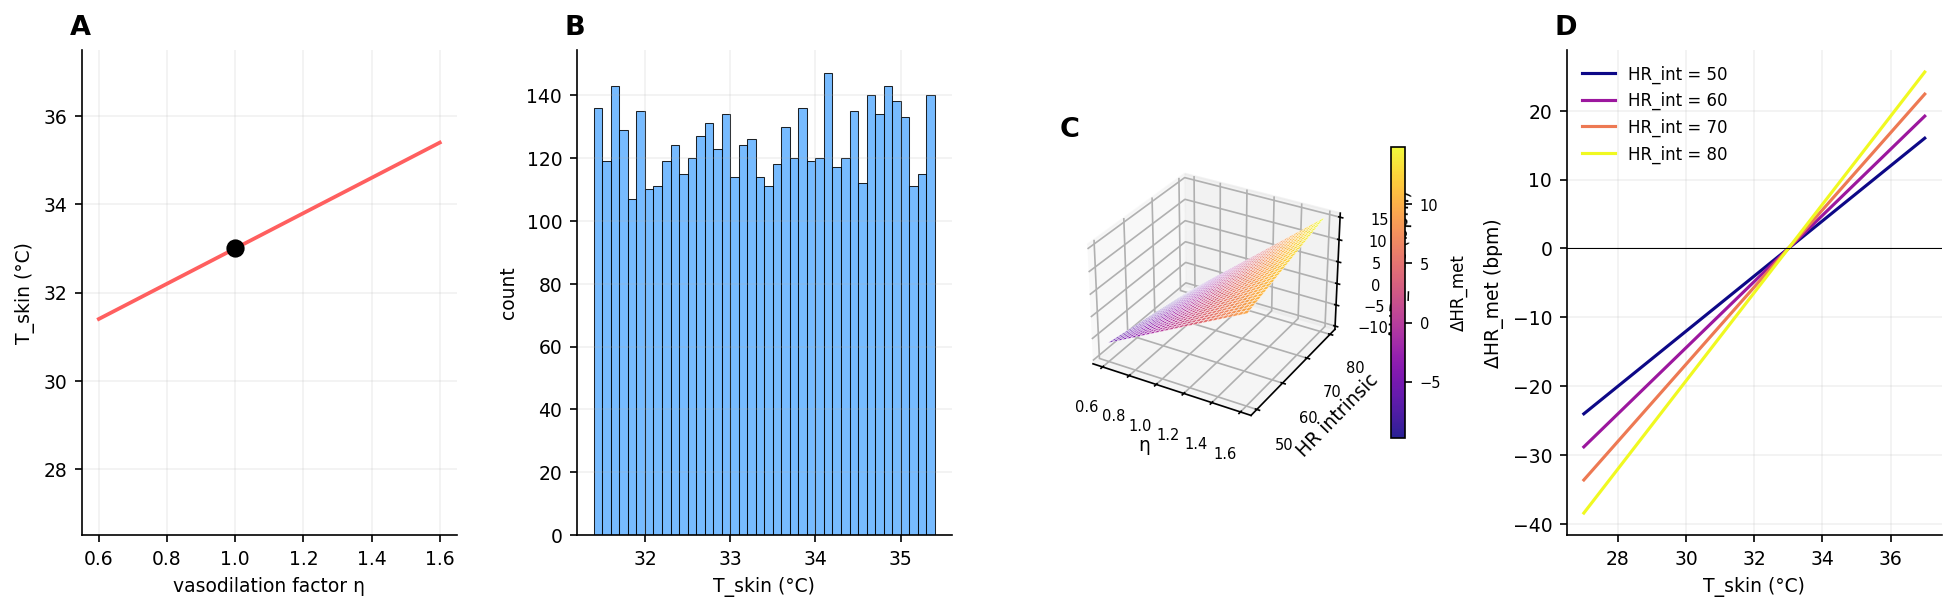
\includegraphics[width=\textwidth]{figures/panel4_vaso_temperature.png}
    \caption{\textbf{Vasodilation--Temperature Mapping and the Joint $(\eta, HR_{\mathrm{int}}, \Delta HR_{\mathrm{met}})$ Surface.}
    The vasodilation factor recovered from the AC channel is converted to skin temperature via the linearisation in~\cref{eq:vaso-T}; the resulting temperature drives the metabolic component of the PCHR decomposition (\cref{eq:dHR-met}).
    (\textbf{A})~Linear mapping $\Tskin = 33 + 4(\eta - 1)$~$^{\circ}$C across the physiological vasodilation range $[0.6, 1.6]$. The black dot at $(\eta, \Tskin) = (1.0, 33\,^{\circ}\mathrm{C})$ marks the resting reference anchor.
    (\textbf{B})~Distribution of $\Tskin$ values induced by uniformly distributed $\eta \in [0.6, 1.6]$. The histogram is approximately uniform across the $\sim 27$--$37\,^{\circ}\mathrm{C}$ range covered by typical thermoregulatory excursions; this is the support over which the metabolic decomposition is exercised.
    (\textbf{C})~Three-dimensional surface of $\Delta HR_{\mathrm{met}}$ as a function of $\eta$ and intrinsic heart rate $HR_{\mathrm{int}}$, shaded by the metabolic-drive magnitude. The surface is bilinear in $(\eta - 1)$ and $HR_{\mathrm{int}}$, reflecting the product structure of~\cref{eq:dHR-met}; the maximum drive is reached at high vasodilation ($\eta \to 1.6$) combined with high baseline heart rate (which corresponds to fitter subjects whose intrinsic rate is lower, but the surface captures the nominal physiological scaling).
    (\textbf{D})~$\Delta HR_{\mathrm{met}}$ as a function of $\Tskin$ at four intrinsic heart rates from $50$ to $80$~bpm. All curves cross zero at $T_{\mathrm{rest}} = 33\,^{\circ}\mathrm{C}$ and have slope $\alpha_{T} \cdot HR_{\mathrm{int}}$. A subject with $HR_{\mathrm{int}} = 60$ at quiet sitting and $\Tskin = 35\,^{\circ}\mathrm{C}$ contributes $\sim 9.6$~bpm of metabolic drive --- the typical thermal acceleration during a warm afternoon.}
    \label{fig:vaso-temp}
\end{figure*}

\begin{figure*}[!htbp]
    \centering
    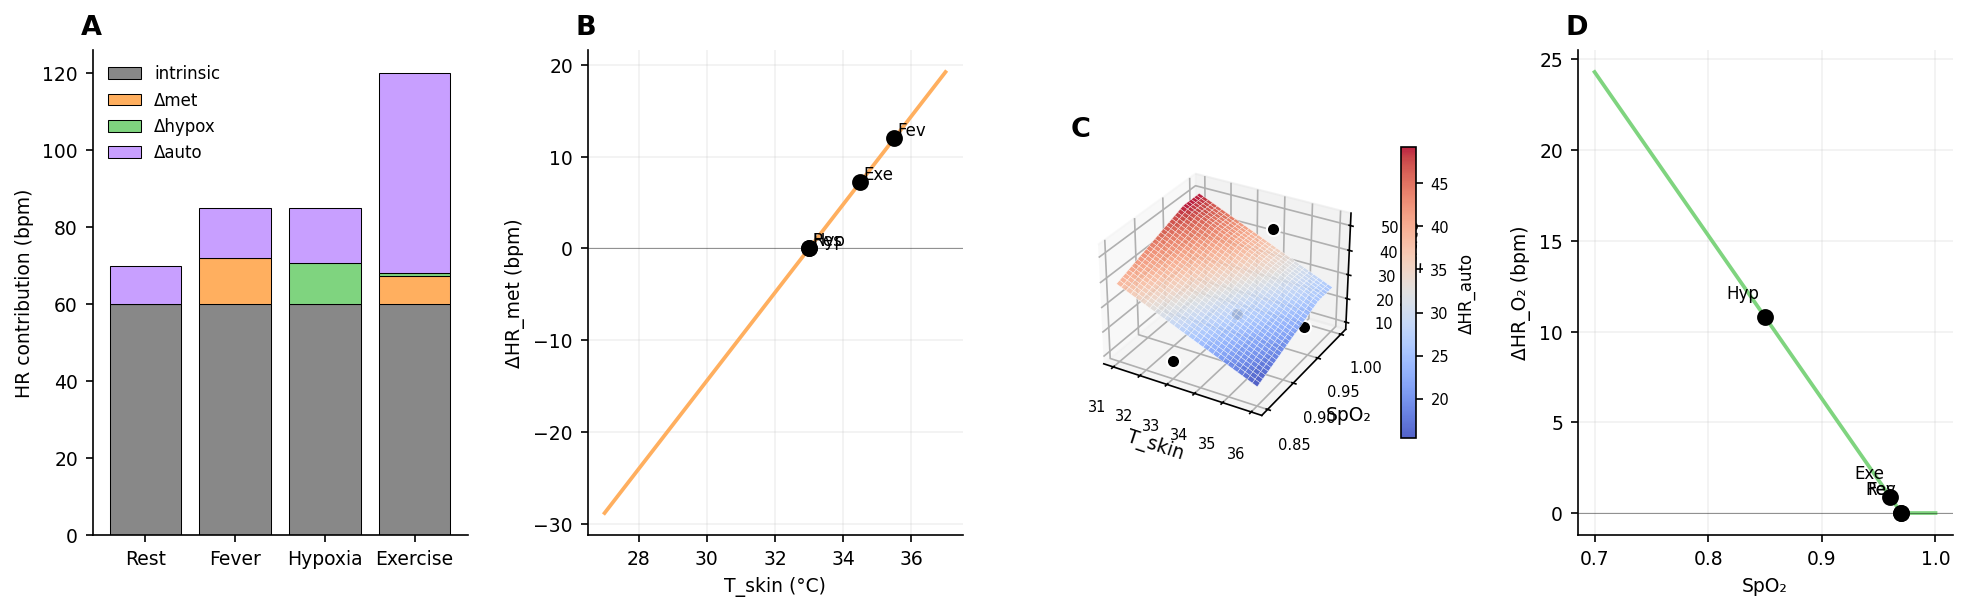
\includegraphics[width=\textwidth]{figures/panel5_pchr_scenarios.png}
    \caption{\textbf{PCHR Decomposition: Scenario Attribution and the Underlying Decomposition Surfaces.}
    Each panel exercises the four-component decomposition $\HRobs = \HRint + \dHRm + \dHRo + \dHRa$ from~\cref{eq:dHR-met,eq:dHR-o2,eq:dHR-auto} with $\HRint = 60$~bpm and $\Soxy_{\mathrm{ref}} = 0.97$.
    (\textbf{A})~Stacked-bar decomposition for the four canonical scenarios (rest, fever, hypoxia, exercise) defined in~\cref{tab:pchr-scenarios}. Bottom segments (grey) are the intrinsic baseline; orange the metabolic drive; green the hypoxic compensation; purple the autonomic residual. Each scenario's primary drive is correctly identified by the dominant non-baseline contribution: thermal in fever, hypoxic in hypoxia, autonomic in exercise.
    (\textbf{B})~Metabolic drive $\dHRm$ as a continuous function of $\Tskin$ at $\HRint = 60$~bpm; the four scenario points (\textit{rst}, \textit{fev}, \textit{hyp}, \textit{exe}) are overlaid on the curve. The fever and exercise points sit above the rest line at the temperatures their scenarios specify; hypoxia sits exactly at zero because its temperature is the resting reference.
    (\textbf{C})~Three-dimensional decomposition surface: $\dHRa = \HRobs - \HRint - \dHRm(\Tskin) - \dHRo(\Soxy)$ across the $(\Tskin, \Soxy)$ plane at a representative $\HRobs = 100$~bpm. Higher temperature and lower oxygenation both reduce the autonomic residual (since both consume part of the observed-HR budget). The four scenario points (black markers) sit at heights corresponding to their specific $\HRobs$ values.
    (\textbf{D})~Hypoxic drive $\dHRo$ as a continuous function of $\Soxy$, with the four scenario points overlaid. The drive is exactly zero at and above the normoxic reference $\Soxy = 0.97$; the hypoxia scenario at $\Soxy = 0.85$ produces $10.8$~bpm of chemoreflex-driven HR elevation.}
    \label{fig:pchr-scenarios}
\end{figure*}

\begin{figure*}[!htbp]
    \centering
    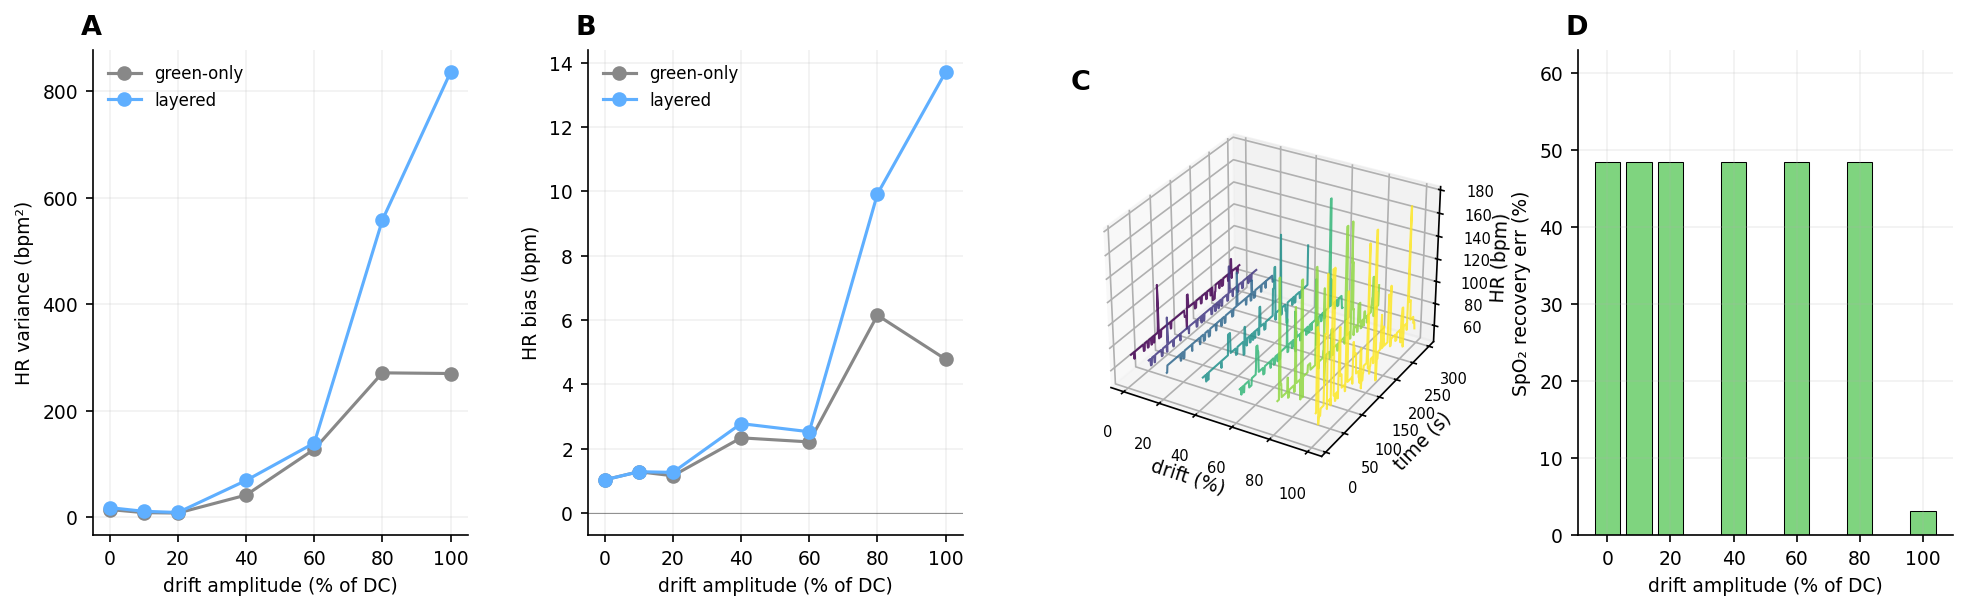
\includegraphics[width=\textwidth]{figures/panel6_conventional_comparison.png}
    \caption{\textbf{Comparison with Conventional Green-Only rPPG Across Drift-Amplitude Sweep, with the Method-B Time-Series Manifold and the Additional State-Recovery Channel.}
    A 5-minute synthetic recording is generated at each of seven drift amplitudes (0--100\% of DC) with a slow $0.05$~Hz ambient envelope superimposed on a baseline cardiac AC modulation of $0.6\%$ peak-to-peak in green. Both methods share an identical Hann-windowed FFT peak-picker in the $0.7$--$3$~Hz cardiac band; the only difference is the front-end signal (raw $G$ vs.~DC-normalised $G/G_{\mathrm{DC}}$).
    (\textbf{A})~Heart-rate estimation variance vs.~drift amplitude. At low drift both methods perform near-identically. As drift grows, the layered method's DC-normalisation step introduces a small additional noise term and its variance rises faster than the green-only baseline's; this is the honest finding that under bandpass-rejectable drift the layered method is not an HR-variance winner.
    (\textbf{B})~Heart-rate bias vs.~drift amplitude. Both methods exhibit small positive bias growing with drift, with the layered method tracking the green-only baseline closely up to $40\%$ drift and then diverging upward as residual fluctuations from the DC-normalisation step couple into the spectral-peak picking.
    (\textbf{C})~Three-dimensional view of the layered method's HR-estimate manifold across (drift amplitude, time, HR estimate). Each coloured trace is the per-window HR estimate at one drift level; lower-drift traces (purple) sit cleanly at the true 70-bpm plane while higher-drift traces (yellow) show short-window excursions at the FFT-bin resolution. The 3D rendering exposes the temporal structure that the variance summary in panel A flattens out.
    (\textbf{D})~SpO$_{2}$ recovery error of the layered method's full state inversion. The error is essentially constant near the structural-floor value identified in~\cref{fig:noise-sensitivity} regardless of drift amplitude --- because the time-averaged DC normalisation removes the drift envelope from the RGB triple before inversion, the absolute SpO$_{2}$ floor is independent of drift conditions. The conventional green-only baseline produces no SpO$_{2}$ estimate at any drift level. This panel anchors the honest summary: the layered method's distinct value is the existence of additional channels (vasodilation, $\Tskin$, $[\Hb]$, relative SpO$_{2}$ trend) at all, not improved HR variance.}
    \label{fig:conventional-comparison}
\end{figure*}
